%******************************************************************************************************
%****************************** Second Chapter ********************************************************
%******************************************************************************************************

\chapter{Literature Review}
\label{litrev}

% **************************** Define Graphics Path **************************
\graphicspath{{Chapter2/Figs/}}
% **************************** Define Graphics Path **************************

Now that we have clearly defined objectives, it is necessary to discuss and analyse existing literature that may help to understand and complete our aims.  
%TODO introduce section properly


%******************************************************************************************************
%******************************************************************************************************
\section{Dubins Paths}
\label{litrev:dubins}
In 1957, an American mathematician by the name of Lester Dubins described what we now refer to as ``Dubins paths'' \cite{dubins1957curves}. A Dubins path described the shortest route for a vehicle between two points under the following conditions:
\begin{itemize}
	\item The curvature of the path is bound by a limit
	\item The vehicle is only able to travel in one direction; forward
	\item The path starts at a position with a given orientation
	\item The path ends at a position with a given orientation
	\item The path is in a 2D plane
\end{itemize}

In the context of this project, the maximum curvature of the path is dictated by the maximum turning rate of the given aircraft, and as such is a hard limit which must be observed for any path planning processes.

The results of Dubins' work was that the shortest path to meet these conditions consisted of three segments, which could be either a left turn segment, a right turn segment, or a straight line segment. These are given the identifiers L, R, and S, respectively. Dubins showed that the shortest available path would always fall under one of the following 6 categories:
\begin{enumerate}
	\item RSR
	\item RSL
	\item RLR
	\item LRL
	\item LSR
	\item LRL
\end{enumerate}

where, for example, RSL refers to a path consisting of a right turn segment, followed by a straight line segment, followed by a left turn segment, as can be seen in Fig. \ref{fig:rsl}. For reference, Fig. \ref{fig:lsl} shows a LSL path example, Fig. \ref{fig:rlr} shows a RLR path example, and Fig. \ref{fig:rsl} shows a RSL path example. 

\begin{figure}[htbp!] 
\centering    
\includegraphics[width=0.5\textwidth]{LSL}
\caption[Dubins LSL Path]{An example LSL Dubins path}
\label{fig:lsl}
\end{figure}

\begin{figure}[htbp!] 
\centering    
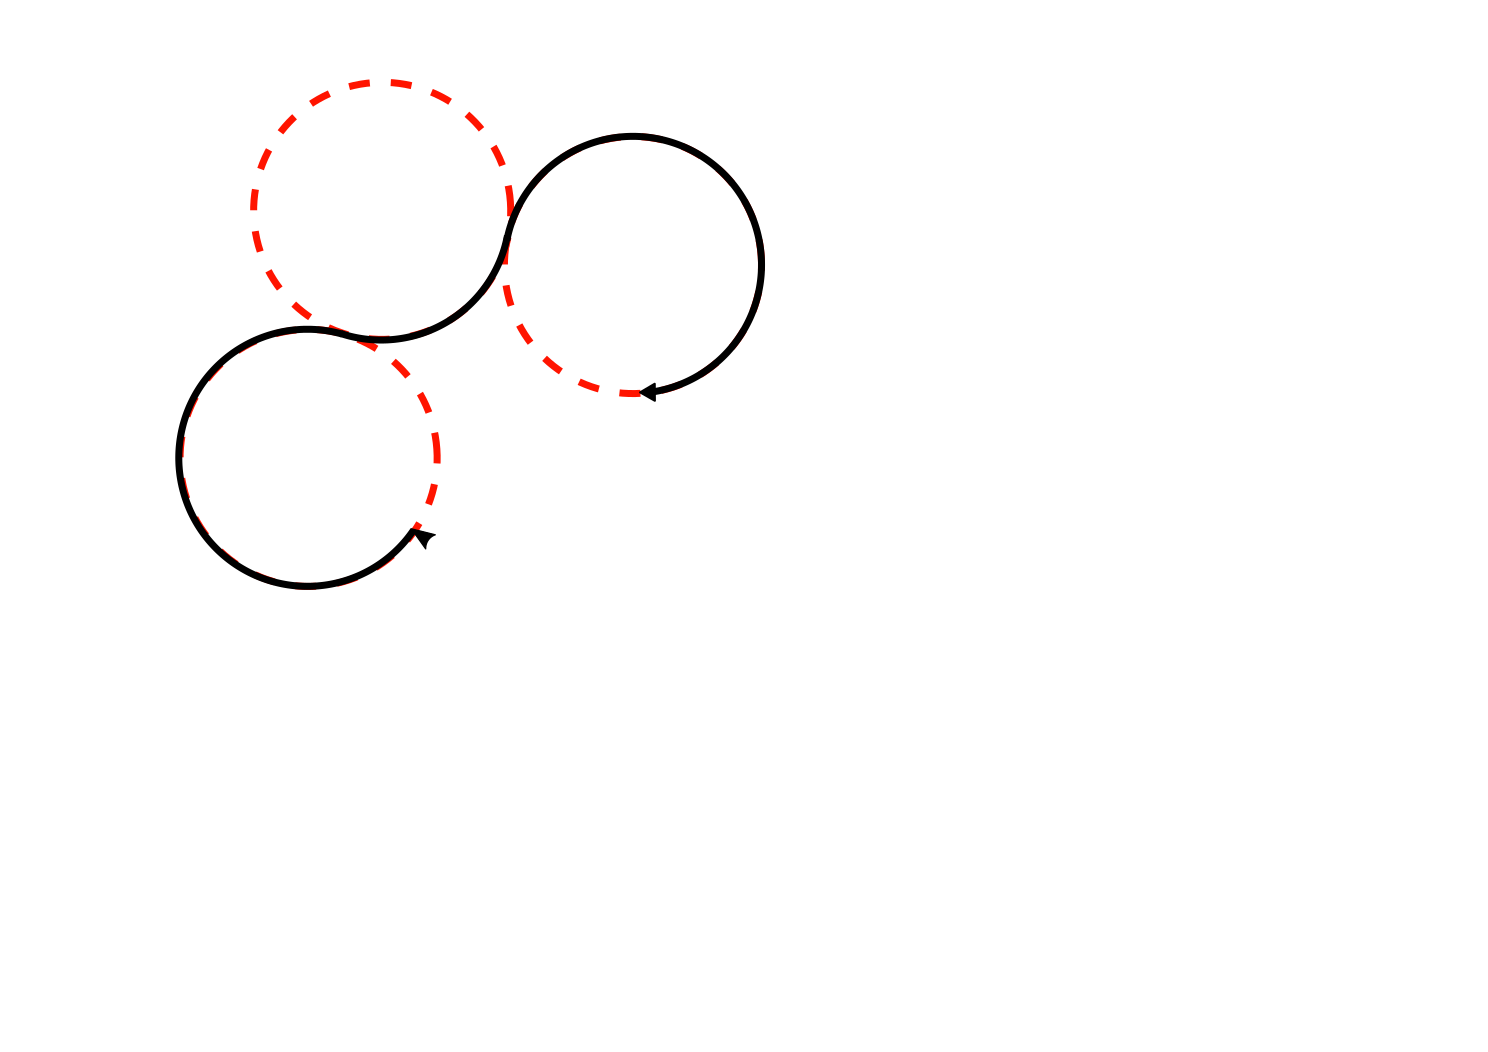
\includegraphics[width=0.5\textwidth]{RLR}
\caption[Dubins RLR Path]{An example RLR Dubins path}
\label{fig:rlr}
\end{figure}

\begin{figure}[htbp!] 
\centering    
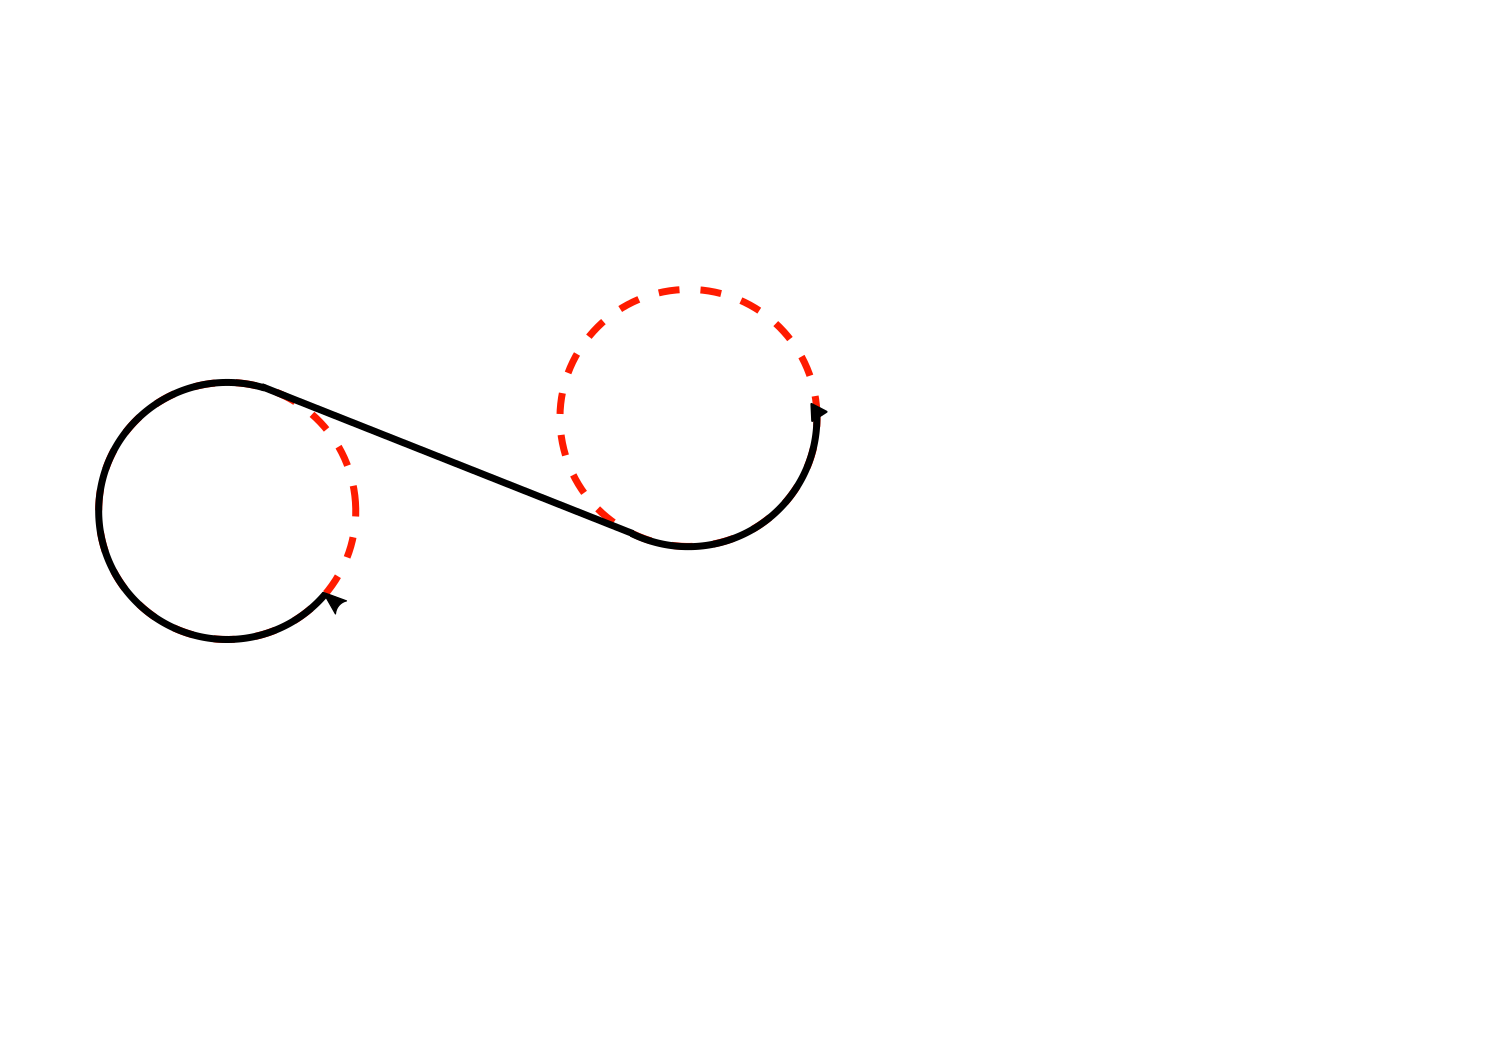
\includegraphics[width=0.5\textwidth]{RSL}
\caption[Dubins RSL Path]{An example RSL Dubins path}
\label{fig:rsl}
\end{figure}

In these diagrams, the arrows show us the initial and final locations, orientations, and direction of travel. The dashed circle in red shows the maximum curvature of any part of the path, which corresponds to a UAV's minumum turning radius. Dubins paths can take many forms, these three examples are intended to enable the reader to visualise their general form and how they relate to the conditions defined above.



%******************************************************************************************************
%******************************************************************************************************
\section{Path Following in Wind}
\label{litrev:path}
